% layouts
% EBS choices
% Geologies


\begin{frame}[ctb!]
  \frametitle{Clay Disposal Environments}

  \begin{figure}[h!]
    \begin{center}
      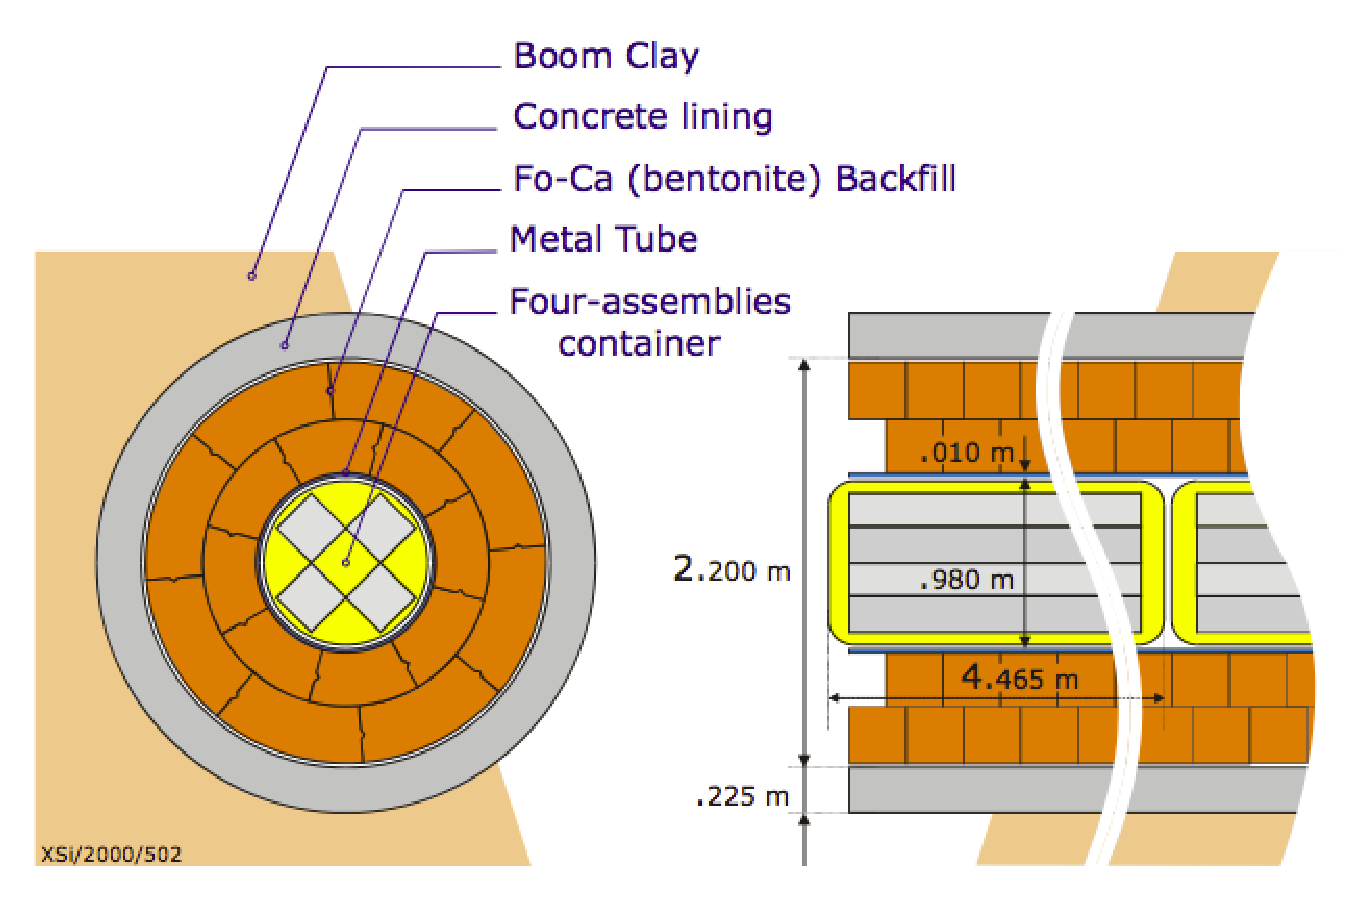
\includegraphics[height=.7\textheight]{belgianClayRedImp.eps}
    \end{center}
    \caption{Belgian reference concept in Boom Clay 
    \cite{von_lensa_red-impact_2008}.}
    \label{fig:belgianClayRedImp}
  \end{figure}

\end{frame}

\begin{frame}[ctb!]
  \frametitle{Granite Disposal Environments}

  \begin{figure}[h!]
    \begin{center}
      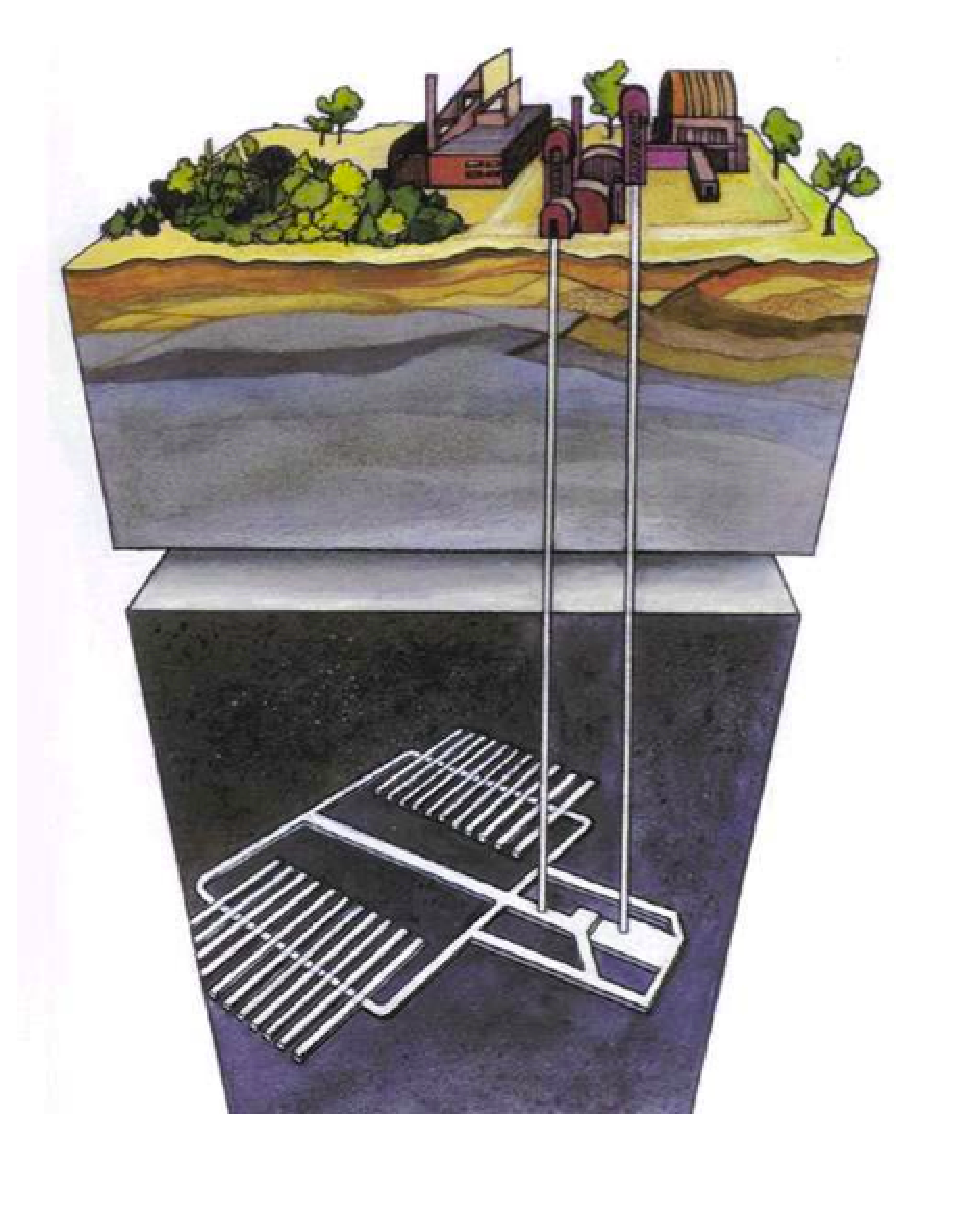
\includegraphics[height=.7\textheight]{czechGraniteRedImp.eps}
    \end{center}
    \caption{Czech reference concept in Granite 
    \cite{von_lensa_red-impact_2008}.}
    \label{fig:czechGraniteRedImp}
  \end{figure}

\end{frame}

\begin{frame}[ctb!]
  \frametitle{Salt Disposal Environments}

  \begin{figure}[h!]
    \begin{center}
      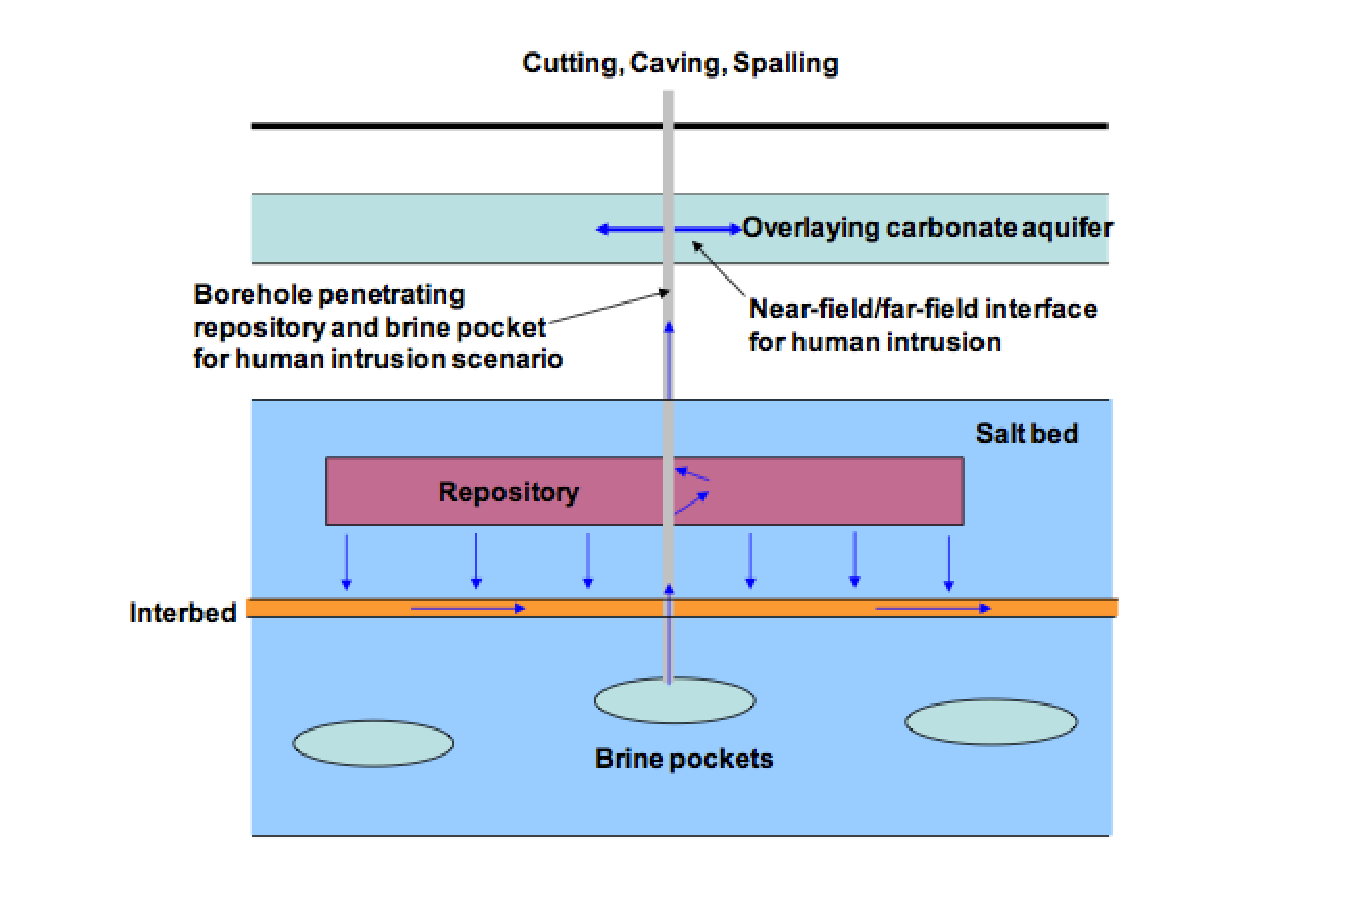
\includegraphics[height=.7\textheight]{saltGPAM.eps}
    \end{center}
    \caption{DOE-NE Used Fuel Disposition Campaign  concept in 
    Salt \cite{clayton_generic_2011}.}
    \label{fig:saltGPAM}
  \end{figure}

\end{frame}

\begin{frame}[ctb!]
  \frametitle{Deep Borehole Disposal Environment}

  \begin{figure}[h!]
    \begin{center}
      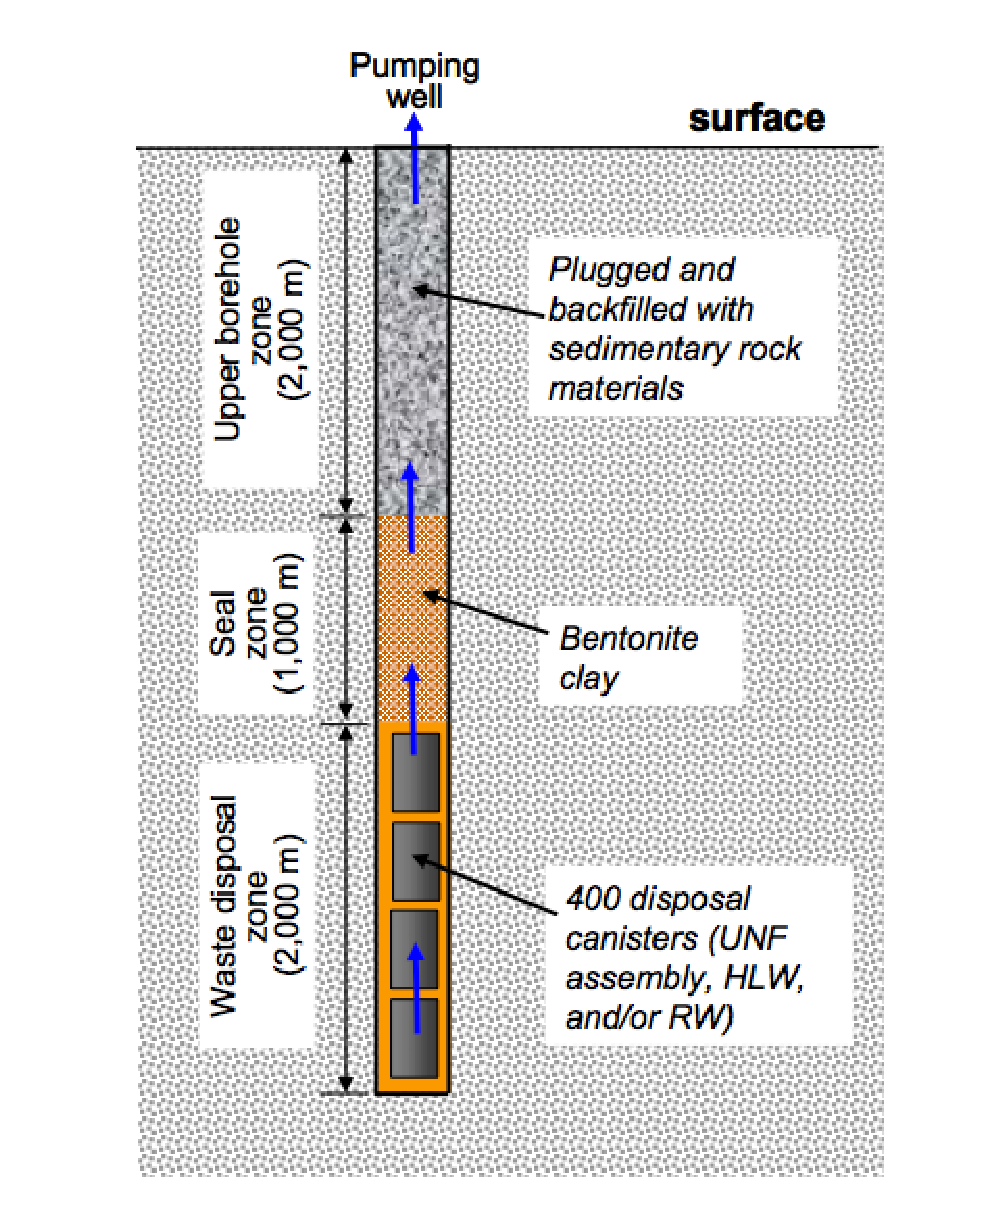
\includegraphics[height=.7\textheight]{boreholeGPAM.eps}
    \end{center}
    \caption{DOE-NE Used Fuel Disposition Campaign Deep Borehole concept 
    \cite{clayton_generic_2011}.}
    \label{fig:boreholeGPAM}
  \end{figure}

\end{frame}


\begin{frame}
  \frametitle{Repository Layouts}

  \begin{minipage}{0.49\textwidth}
    \begin{figure}[h!]
      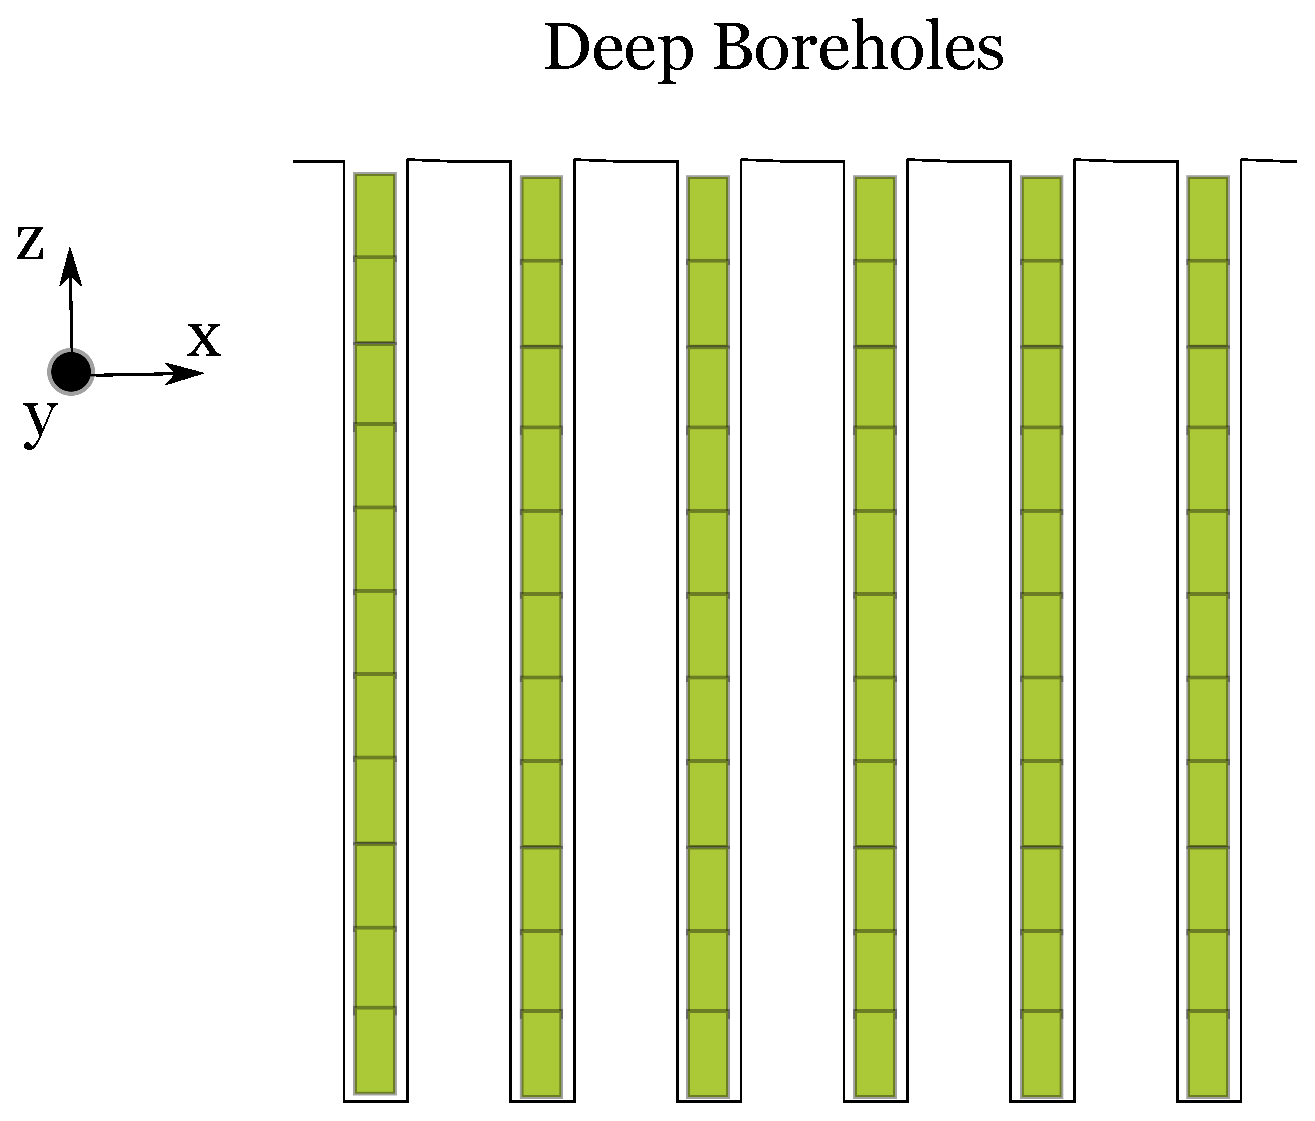
\includegraphics[width=0.75\textwidth]{boreholes.eps}
    \end{figure}
    \begin{figure}[h!]
      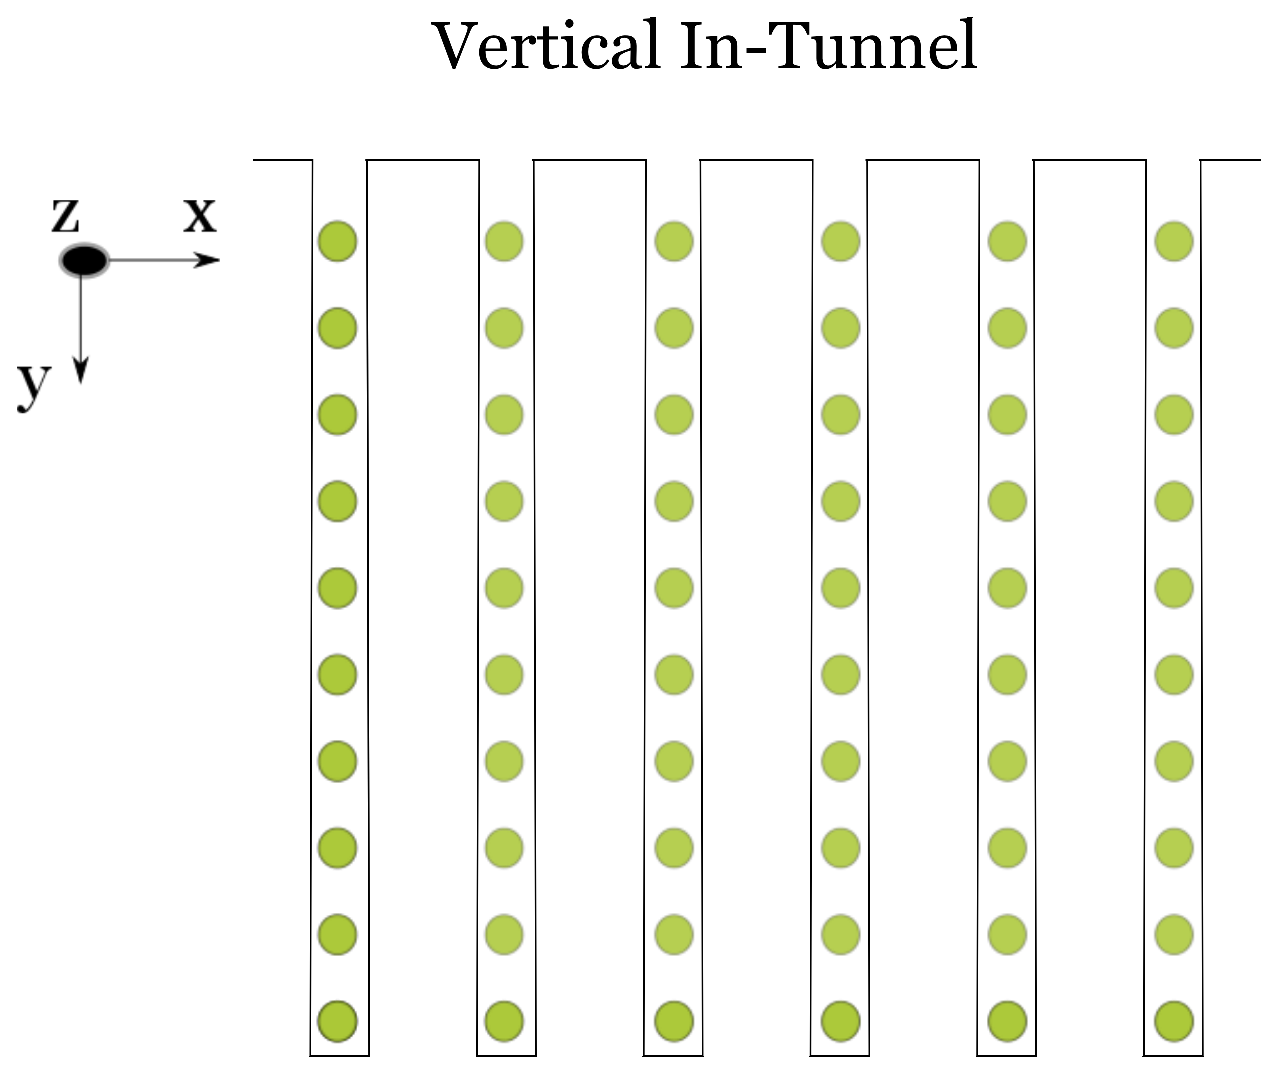
\includegraphics[width=0.75\textwidth]{vertical.eps}
    \end{figure}
  \end{minipage}
  \hspace{0.01cm}
  \begin{minipage}{0.49\textwidth}
    \begin{figure}[h!]
      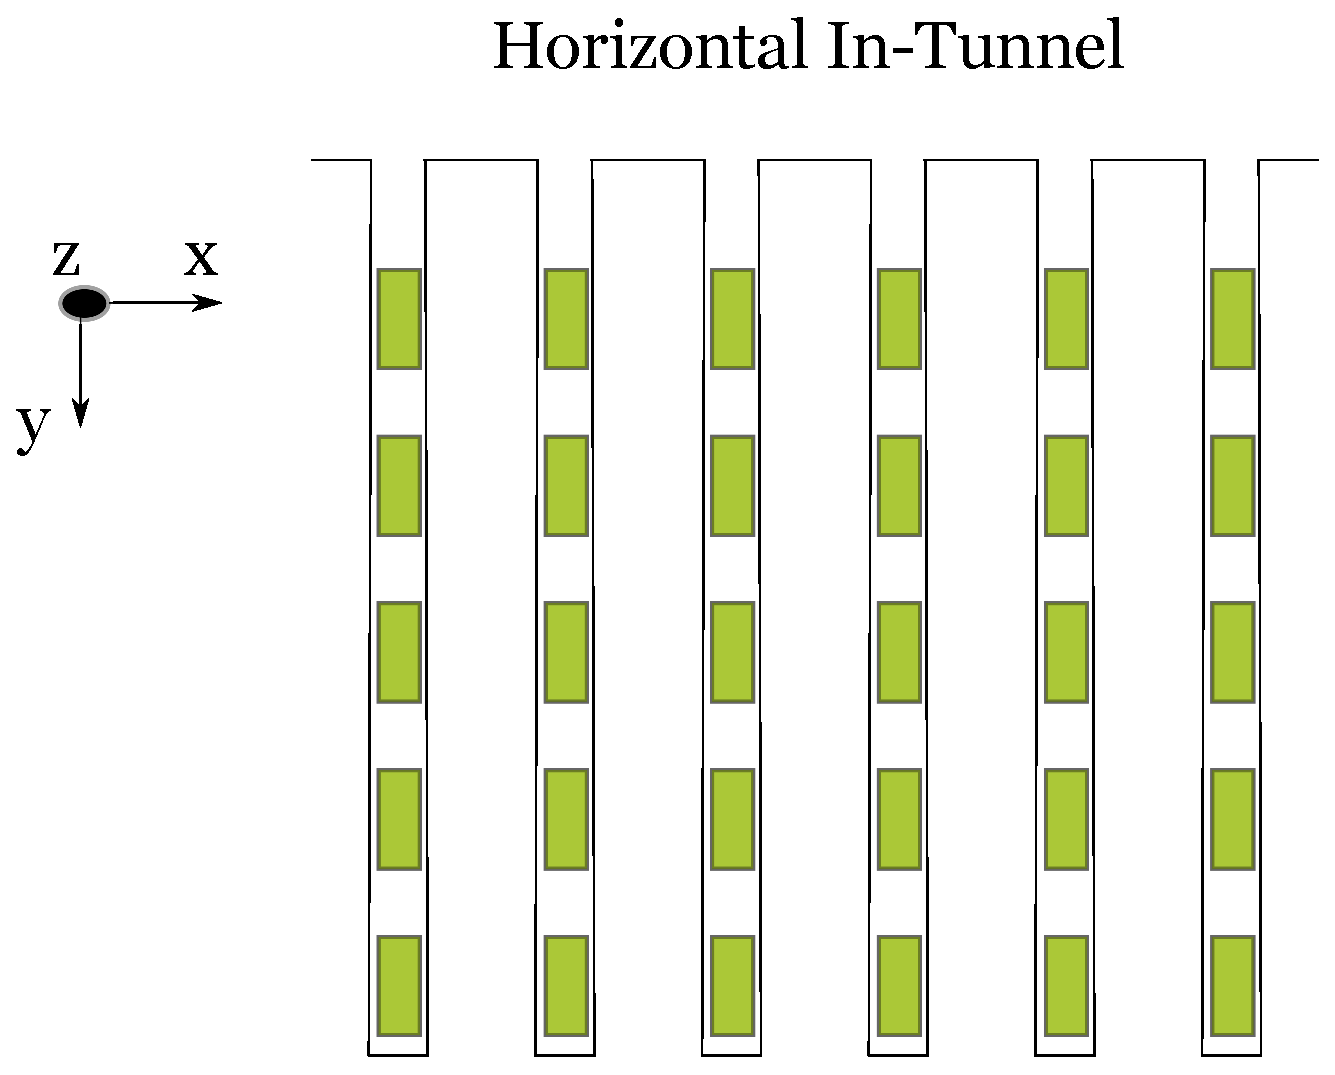
\includegraphics[width=0.8\textwidth]{horizontal.eps}
    \end{figure}
    \begin{figure}[h!]
      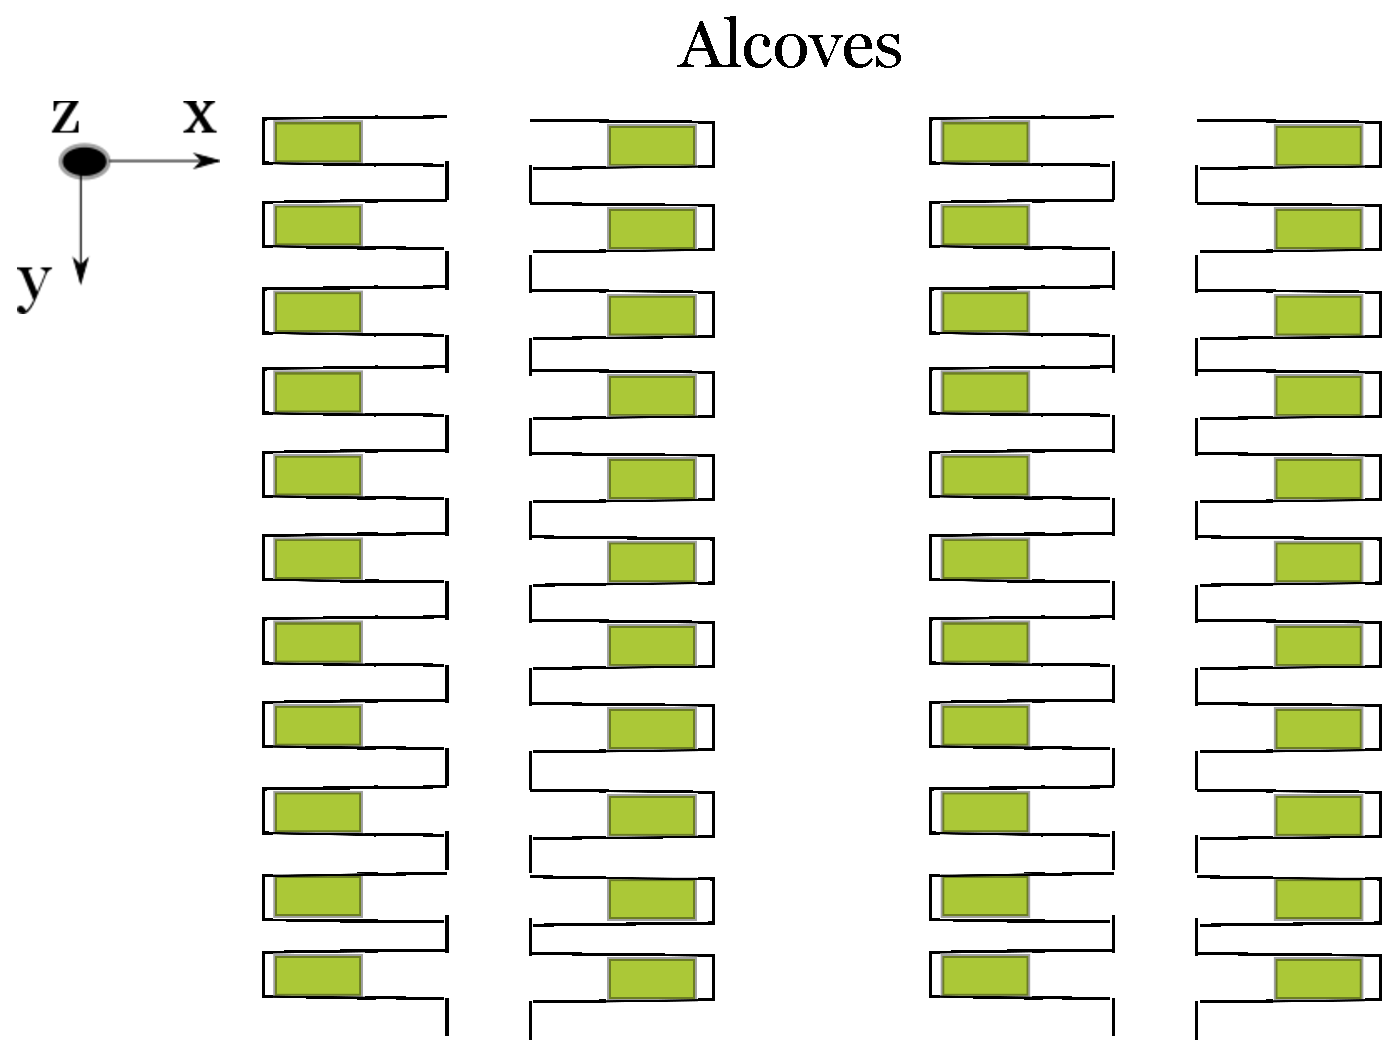
\includegraphics[width=0.8\textwidth]{alcoves.eps}
    \end{figure}
  \end{minipage}

\end{frame}

\begin{frame}[ctb!]
  \frametitle{All Disposal Environments}
  % Table
  %        File: geos_tab.tex
%     Created: Thu Aug 04 11:00 AM 2011 C
% Last Change: Thu Aug 04 11:00 AM 2011 C
%
\begin{table}[h!]
  \centering
  \footnotesize{
  \begin{tabular}{|l|r|r|r|r|}
    \multicolumn{5}{c}{\textbf{Thermal Behavior of Various Concepts}}\\
    \hline
    Feature & Clay & Granite & Salt & Deep Borehole \\ 
    \hline
    Host Rock Limit $[^{\circ}C]$ & $\sim125$ & $\sim200$ & $\sim180$ & $>200$ \\ 
    Buffer Limit $[^{\circ}C]$ & 100 (Fo-Ca) & 100 (Fo-Ca) & 180 & 100 (Fo-Ca)\\ 
    Conductivity $[\frac{W}{m{\cdot}K}]$ & $1-2$ & $2-4$ & $\sim4$  & $2-4$ \\ 
    Diffusivity $[\frac{m^2}{s}]$ & $1-6\times10^{-7}$ & $1\times10^{-6}$ & $1-2\times10^{-6}$  & $1\times10^{-6}$ \\ 
    Coalesence & yes & no & yes & no \\ 
    \hline
  \end{tabular}
  \caption{Reference values for thermal limits and behaviors in various 
  candidate repository geologies.}
  }
  \label{tab:geos_tab}
\end{table}
%  \cite{stober_hydraulic_2006} 

\end{frame}

